\documentclass[11pt, a4paper]{article}
\usepackage{fontspec}
\usepackage{geometry}
\usepackage{booktabs}
\usepackage{graphicx}
\usepackage{xcolor}
\usepackage{titlesec}
\usepackage{enumitem}
\usepackage{caption}
\usepackage{subcaption}
\usepackage{parskip}

\geometry{margin=2.5cm}

\definecolor{accent}{RGB}{30, 80, 160}

\titleformat{\section}{\large\bfseries\color{accent}}{}{0em}{}[\titlerule]
\titleformat{\subsection}{\normalsize\bfseries}{}{0em}{}

\setlist[itemize]{noitemsep, topsep=2pt}

\begin{document}

\begin{center}
  {\LARGE \textbf{Sequential Genetic Testing — Methodology}}\\[0.4em]
  {\large What We Tested, Against What, and Why}\\[0.2em]
  {\small Rana Lab $\cdot$ June 2026}
\end{center}

\vspace{0.5em}
\hrule
\vspace{1em}

%------------------------------------------------------------------
\section{The Problem in One Paragraph}

A family member tests positive for a hereditary cancer gene (e.g.\ BRCA1/2).
The doctor now needs to decide \textbf{who else in the family to test, and in what order}.
Each test costs money. Each result updates your beliefs about everyone else.
The goal is to find carriers efficiently — minimising cost while maximising detection.
This is a sequential decision problem. The exact optimal solution requires enumerating
every possible belief state the doctor could be in, which explodes combinatorially:
9 people = 262,144 states; 15 people = over 1 billion. It is infeasible at clinical scale.

%------------------------------------------------------------------
\section{The Three Methods}

\begin{itemize}
  \item \textbf{Exact DP (Dynamic Programming)} — brute-force backward induction.
        Enumerates every belief state, computes the provably optimal policy.
        Used as \emph{ground truth} to grade everything else.
        Breaks above $\sim$9 family members.

  \item \textbf{ABCD-16 (lab's existing model)} — Approximate Dynamic Programming
        with 16 hand-crafted features (carrier probabilities, pedigree topology,
        test margins). Solves a linear program instead of full DP.
        We replicated this to verify our exact DP solver is correct.

  \item \textbf{RL Agent (our contribution)} — a PPO-trained neural network
        that learns a testing policy by playing the game millions of times.
        Never enumerates states. Runs at constant speed regardless of family size.
\end{itemize}

%------------------------------------------------------------------
\section{The RL Model: PPO + MLP Actor-Critic}

We use \textbf{PPO (Proximal Policy Optimization)} with an \textbf{MLP (Multi-Layer Perceptron) actor-critic} network.

\textbf{What this means:}
\begin{itemize}
  \item \textbf{MLP} — a standard neural network. Takes the current belief state
        (carrier probabilities for each family member + their test status) as input,
        and outputs which person to test next, or to stop.
  \item \textbf{Actor-critic} — two heads on the same network: the \emph{actor}
        picks the action, the \emph{critic} estimates how good the current state is.
        The critic's estimate is used to reduce variance during training.
  \item \textbf{PPO} — the training algorithm. Runs thousands of episodes, collects
        rewards and penalties, and nudges the network weights to make better decisions.
        Same algorithm used in OpenAI's RLHF training for early ChatGPT.
\end{itemize}

\textbf{Why PPO:}
\begin{itemize}
  \item \textbf{Stable} — has a built-in clipping mechanism that prevents the policy
        from changing too drastically in one update, avoiding catastrophic forgetting
  \item \textbf{Works for discrete action spaces} — our action space is discrete:
        test person 1, 2, 3\ldots or stop. PPO handles this naturally
  \item \textbf{Battle-tested and easy to tune} — the default go-to for RL on
        sequential decision problems; reliable results without extensive hyperparameter search
\end{itemize}

\textbf{Note:} the codebase also has a \textbf{GNN (Graph Neural Network)} option
that treats the family pedigree as a graph and could learn structural patterns across
different family shapes. This was built but kept as secondary — not used in the main experiments.

%------------------------------------------------------------------
\section{Experiments Run}

\subsection{1 — RL vs Exact DP: Optimality Gap}
\textit{Script: \texttt{benchmark.py} $\cdot$ Figure: fig2, fig7}

Trained RL separately on family sizes N=4, 6, 7, 9. Compared RL reward to exact DP
reward to measure how far RL is from perfect. Also ran RL inference on N=12, 15
where exact DP cannot run at all.

\textbf{Why:} establishes whether RL is a credible approximation of the optimal policy.

\begin{center}
\small
\begin{tabular}{lrrrr}
\toprule
\textbf{Family size} & \textbf{Exact DP states} & \textbf{Exact DP time} & \textbf{RL gap from optimal} & \textbf{RL inference} \\
\midrule
N=4  & 256           & 0.015s   & 16.7\% & 0.12ms \\
N=6  & 4,096         & 3.4s     & 14.6\% & 0.12ms \\
N=7  & 16,384        & 2.1s     & 7.2\%  & 0.13ms \\
N=9  & 262,144       & 61.8s    & 0.5\%  & 0.12ms \\
N=12 & 16,777,216    & infeasible & ---  & 0.11ms \\
N=15 & 1,073,741,824 & infeasible & ---  & 0.12ms \\
\bottomrule
\end{tabular}
\end{center}

\begin{figure}[h]
  \centering
  \begin{subfigure}[t]{0.48\textwidth}
    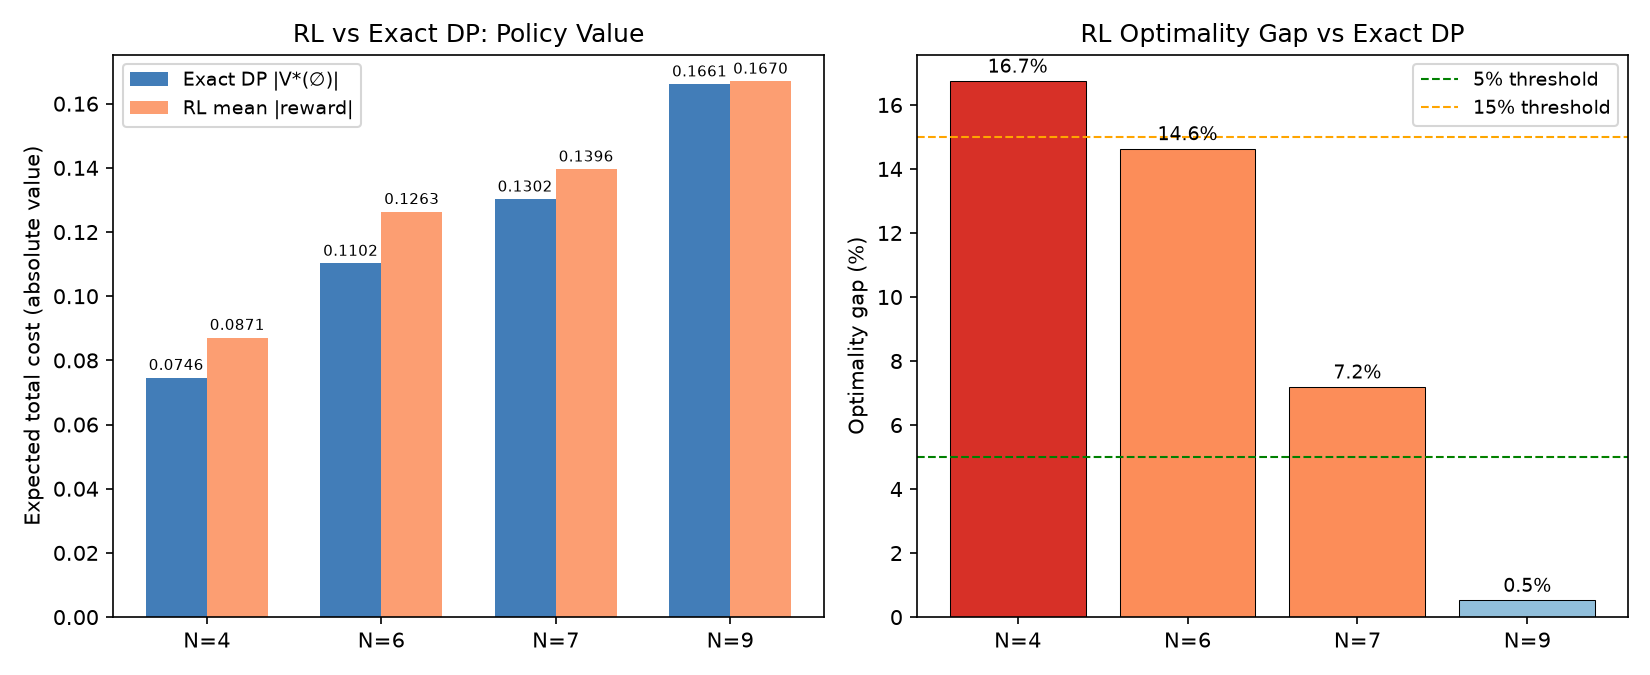
\includegraphics[width=\linewidth]{../artifacts/fig2_optimality_gap.png}
    \caption{Optimality gap vs family size}
  \end{subfigure}
  \hfill
  \begin{subfigure}[t]{0.48\textwidth}
    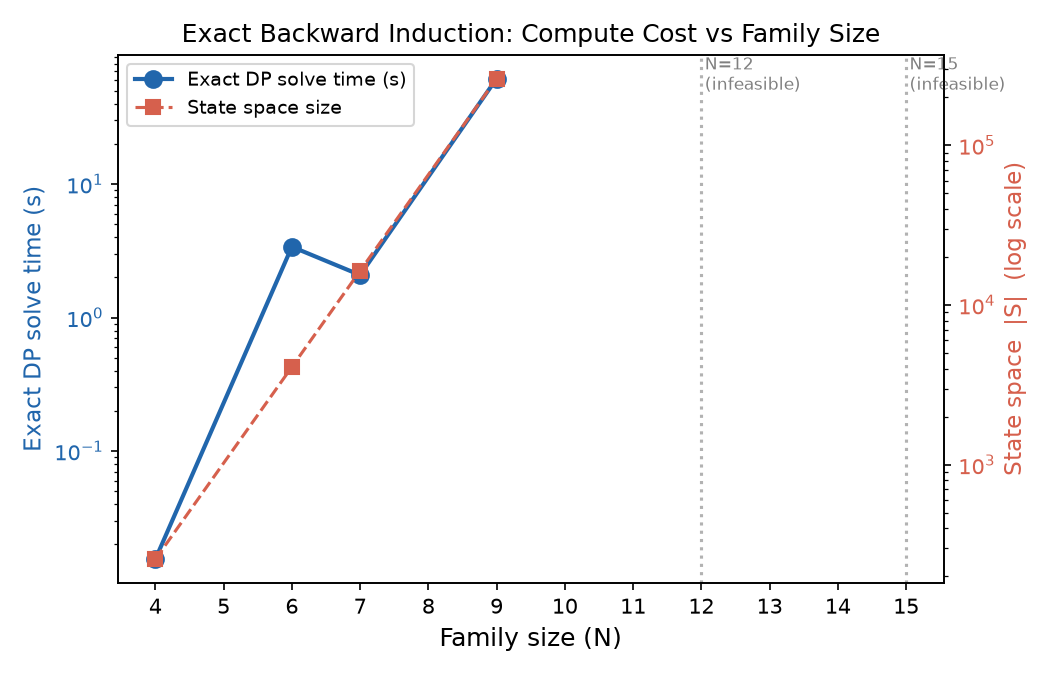
\includegraphics[width=\linewidth]{../artifacts/fig1_compute_time.png}
    \caption{Compute time: exact DP vs RL}
  \end{subfigure}
\end{figure}

\subsection{2 — Scalability: Family Size and Gene Count}
\textit{Script: \texttt{benchmark\_scale.py} $\cdot$ Figure: fig3, fig5, fig6}

Pushed family size from N=4 to N=15 and gene count from G=1 to G=3 on a fixed N=9 family.
Exact DP is run where feasible; RL runs at all sizes.

\textbf{Why:} demonstrates that RL scales where exact DP breaks — the core practical argument.

\begin{figure}[h]
  \centering
  \begin{subfigure}[t]{0.48\textwidth}
    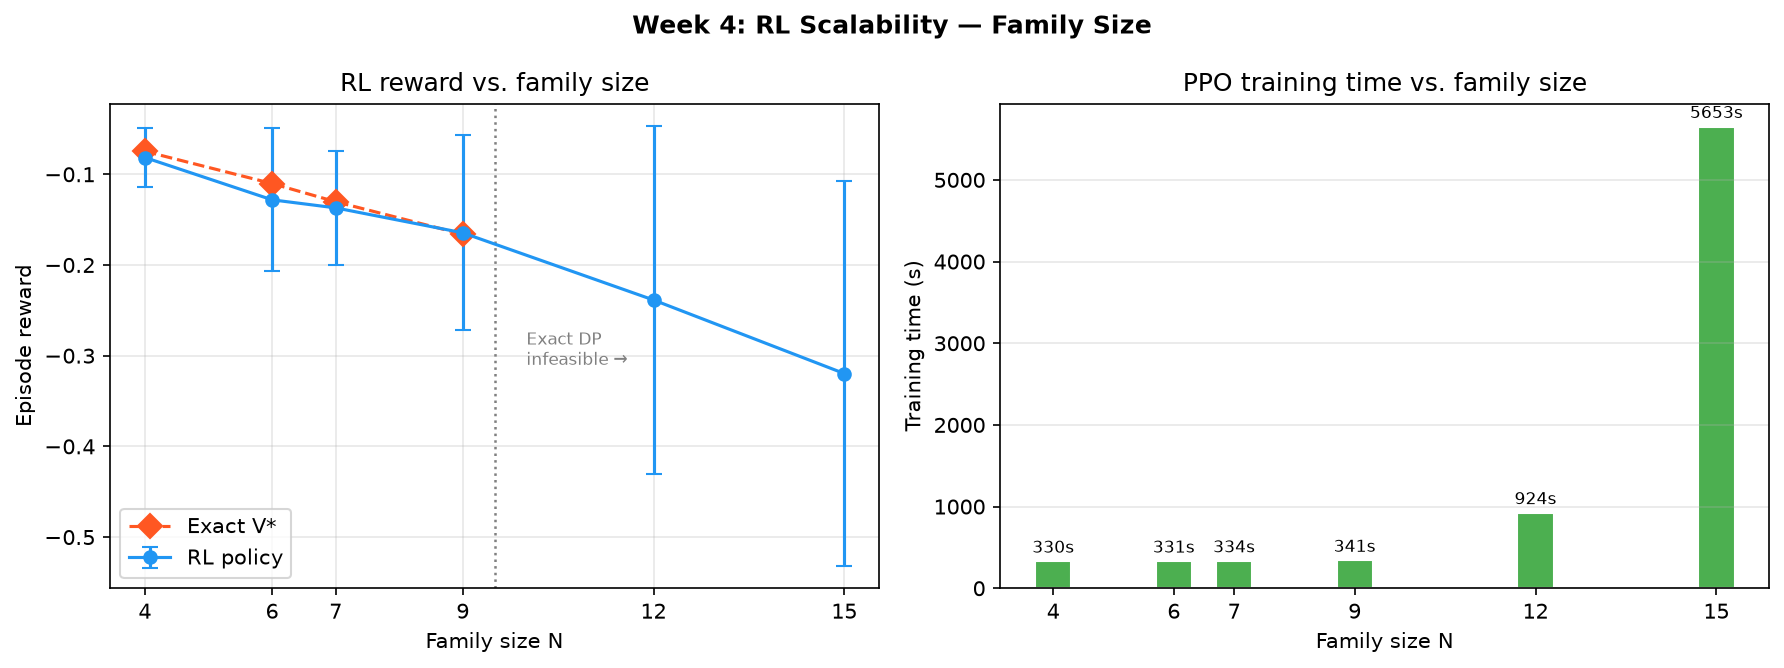
\includegraphics[width=\linewidth]{../artifacts/fig5_family_scale.png}
    \caption{Scaling by family size}
  \end{subfigure}
  \hfill
  \begin{subfigure}[t]{0.48\textwidth}
    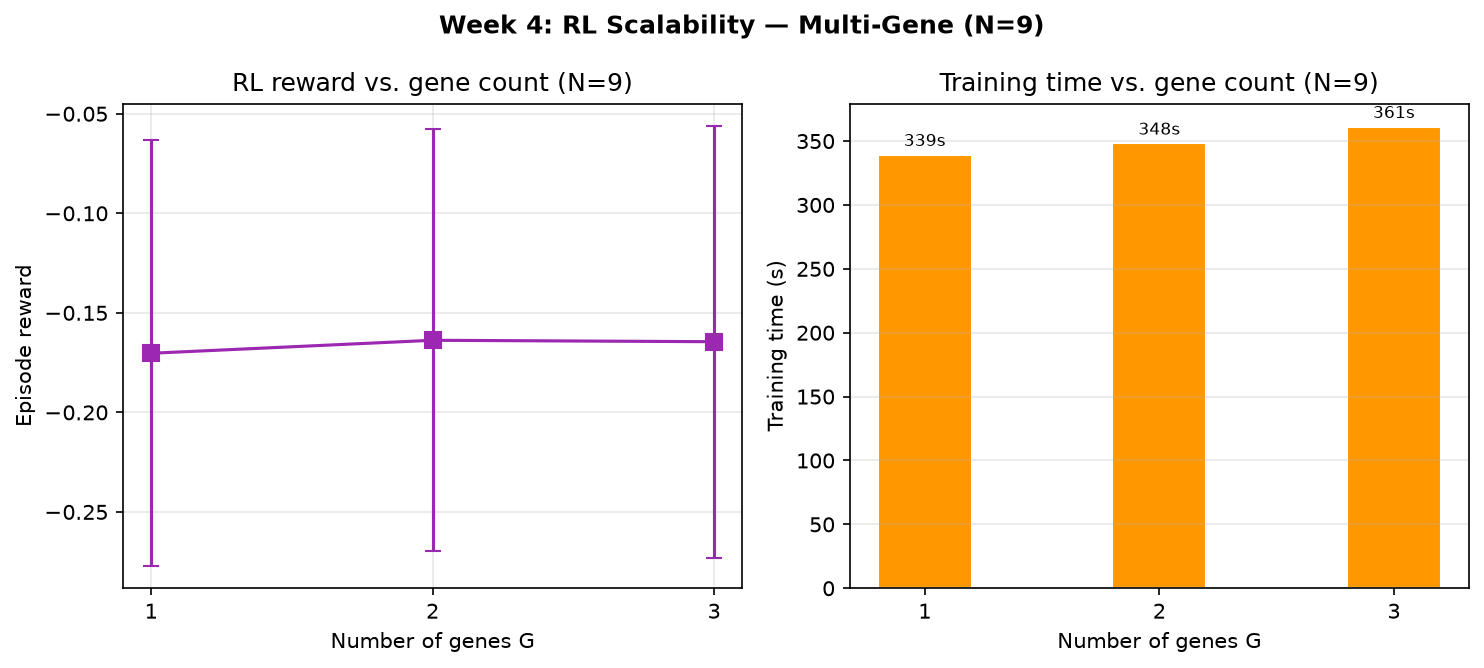
\includegraphics[width=\linewidth]{../artifacts/fig6_multigene.png}
    \caption{Scaling by gene count}
  \end{subfigure}
\end{figure}

\subsection{3 — Baseline Comparison: RL vs Random vs Myopic}
\textit{Script: \texttt{eval\_baselines.py} $\cdot$ Figure: fig8}

Ran RL against three baselines on N=4, 6, 7, 9 over 500 evaluation episodes.
Reward closer to 0 = better (less total penalty incurred).

\textbf{Why:} positions RL relative to simple strategies — random (floor) and
myopic greedy (a strong heuristic that always tests the most suspicious person now,
no forward planning).

\begin{center}
\small
\begin{tabular}{lrrrr}
\toprule
\textbf{Family size} & \textbf{Exact (perfect)} & \textbf{Random} & \textbf{Myopic greedy} & \textbf{RL} \\
\midrule
N=4 & -0.0746 & -0.1243 & -0.0849 & -0.0783 \\
N=6 & -0.1102 & -0.1992 & -0.1245 & -0.1162 \\
N=7 & -0.1302 & -0.2111 & -0.1403 & -0.1316 \\
N=9 & -0.1661 & -0.2828 & -0.1668 & -0.1790 \\
\bottomrule
\end{tabular}
\end{center}

\begin{figure}[h]
  \centering
  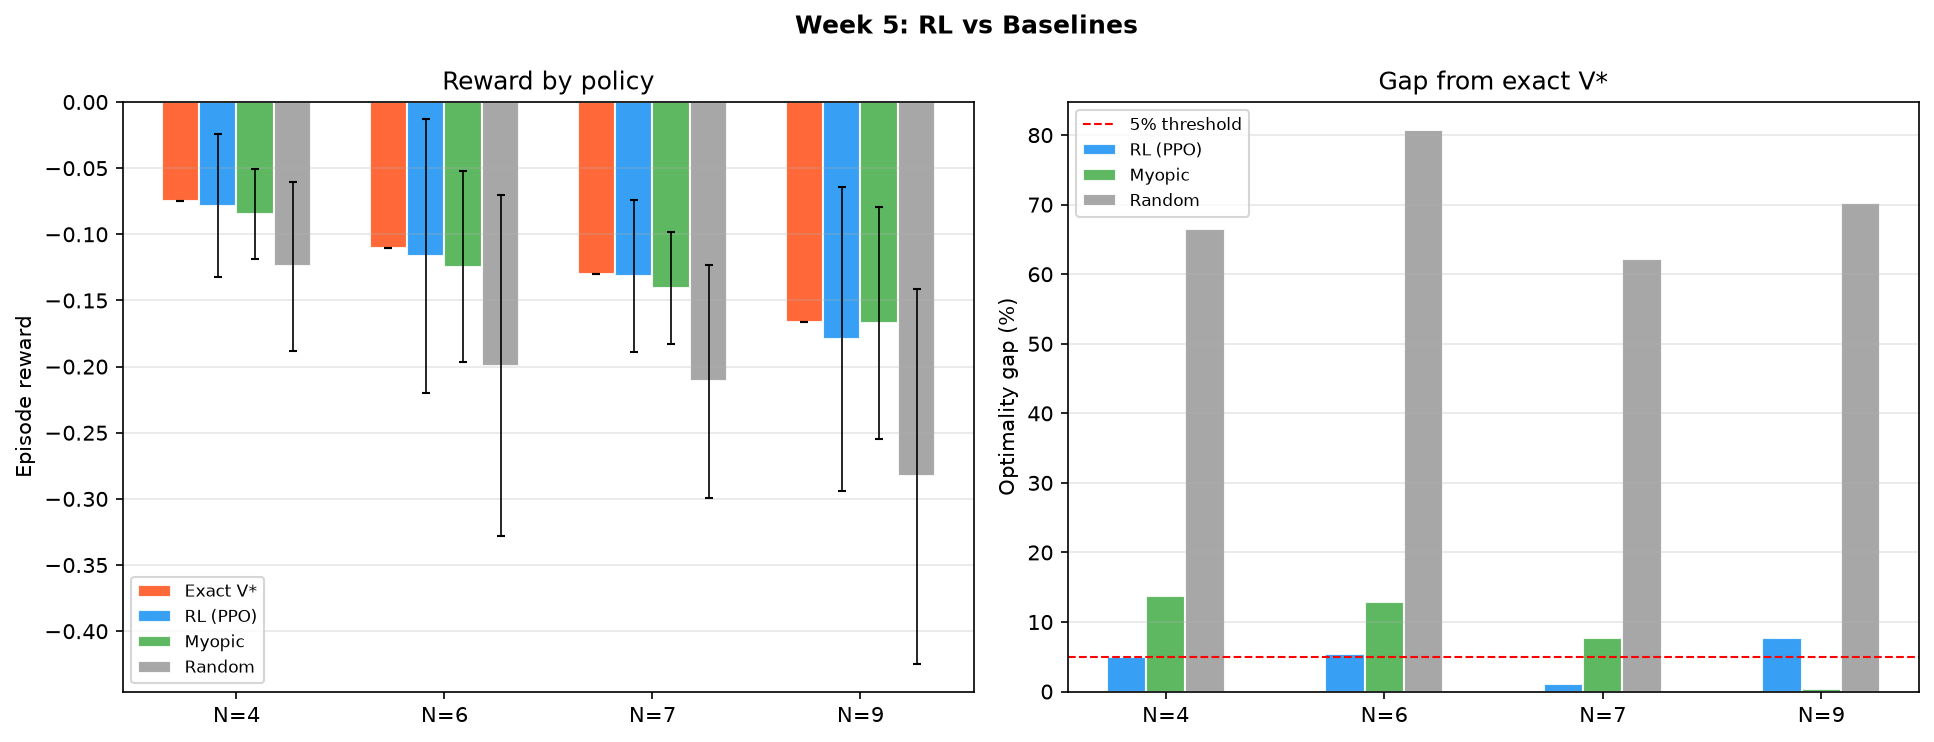
\includegraphics[width=0.6\linewidth]{../artifacts/fig8_baselines.png}
  \caption{Baseline comparison across family sizes}
\end{figure}

\subsection{4 — Sensitivity Analysis: Robustness Across Disease Prevalences}
\textit{Script: \texttt{sensitivity.py} $\cdot$ Figure: fig9}

Fixed N=9, varied allele frequency from 0.05 to 0.30 (covering rare to common
hereditary mutations, including the BRCA1/2 range).

\textbf{Why:} checks whether RL is brittle — if it only works at one prevalence
level, it is not clinically useful.

\textbf{Result:} RL gap from optimal stays between 0.5\% and 9.3\% across the
full range. Robust.

\begin{figure}[h]
  \centering
  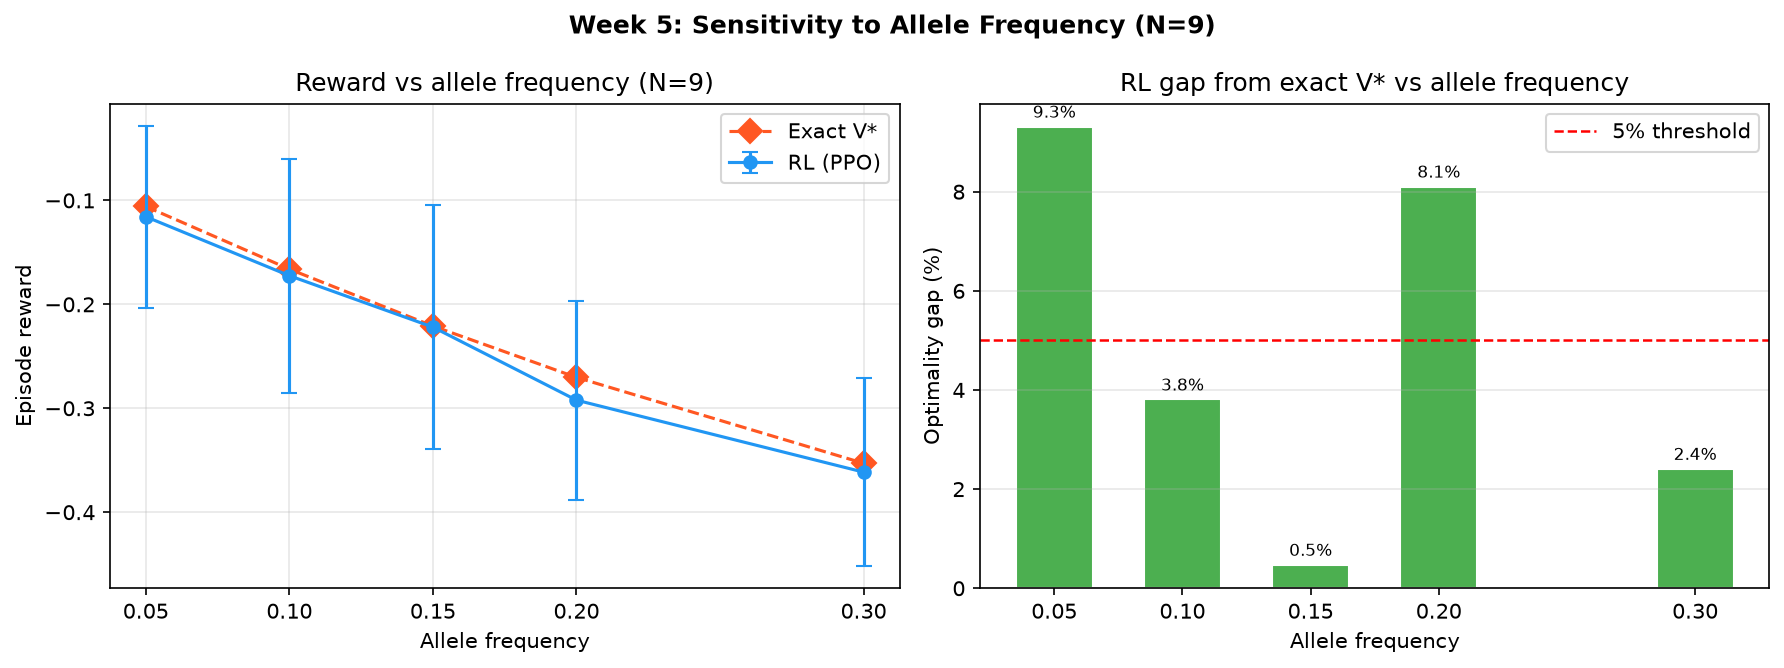
\includegraphics[width=0.6\linewidth]{../artifacts/fig9_sensitivity.png}
  \caption{RL optimality gap across allele frequencies (N=9)}
\end{figure}

\subsection{5 — Policy Behaviour: How Does RL Actually Decide?}
\textit{Script: \texttt{visualize\_policy.py} $\cdot$ Figure: fig10}

Ran 2,000 episodes comparing RL vs myopic greedy on a 9-person family.
Tracked number of tests run per episode and when each policy stops.

\textbf{Why:} reward numbers alone do not tell you \emph{how} the policy behaves.
This checks whether RL is doing something sensible — not just getting lucky.

\textbf{Result:} RL averages 6.05 tests per episode vs myopic's 6.70.
RL is more selective — it stops earlier without sacrificing detection quality.

\begin{figure}[h]
  \centering
  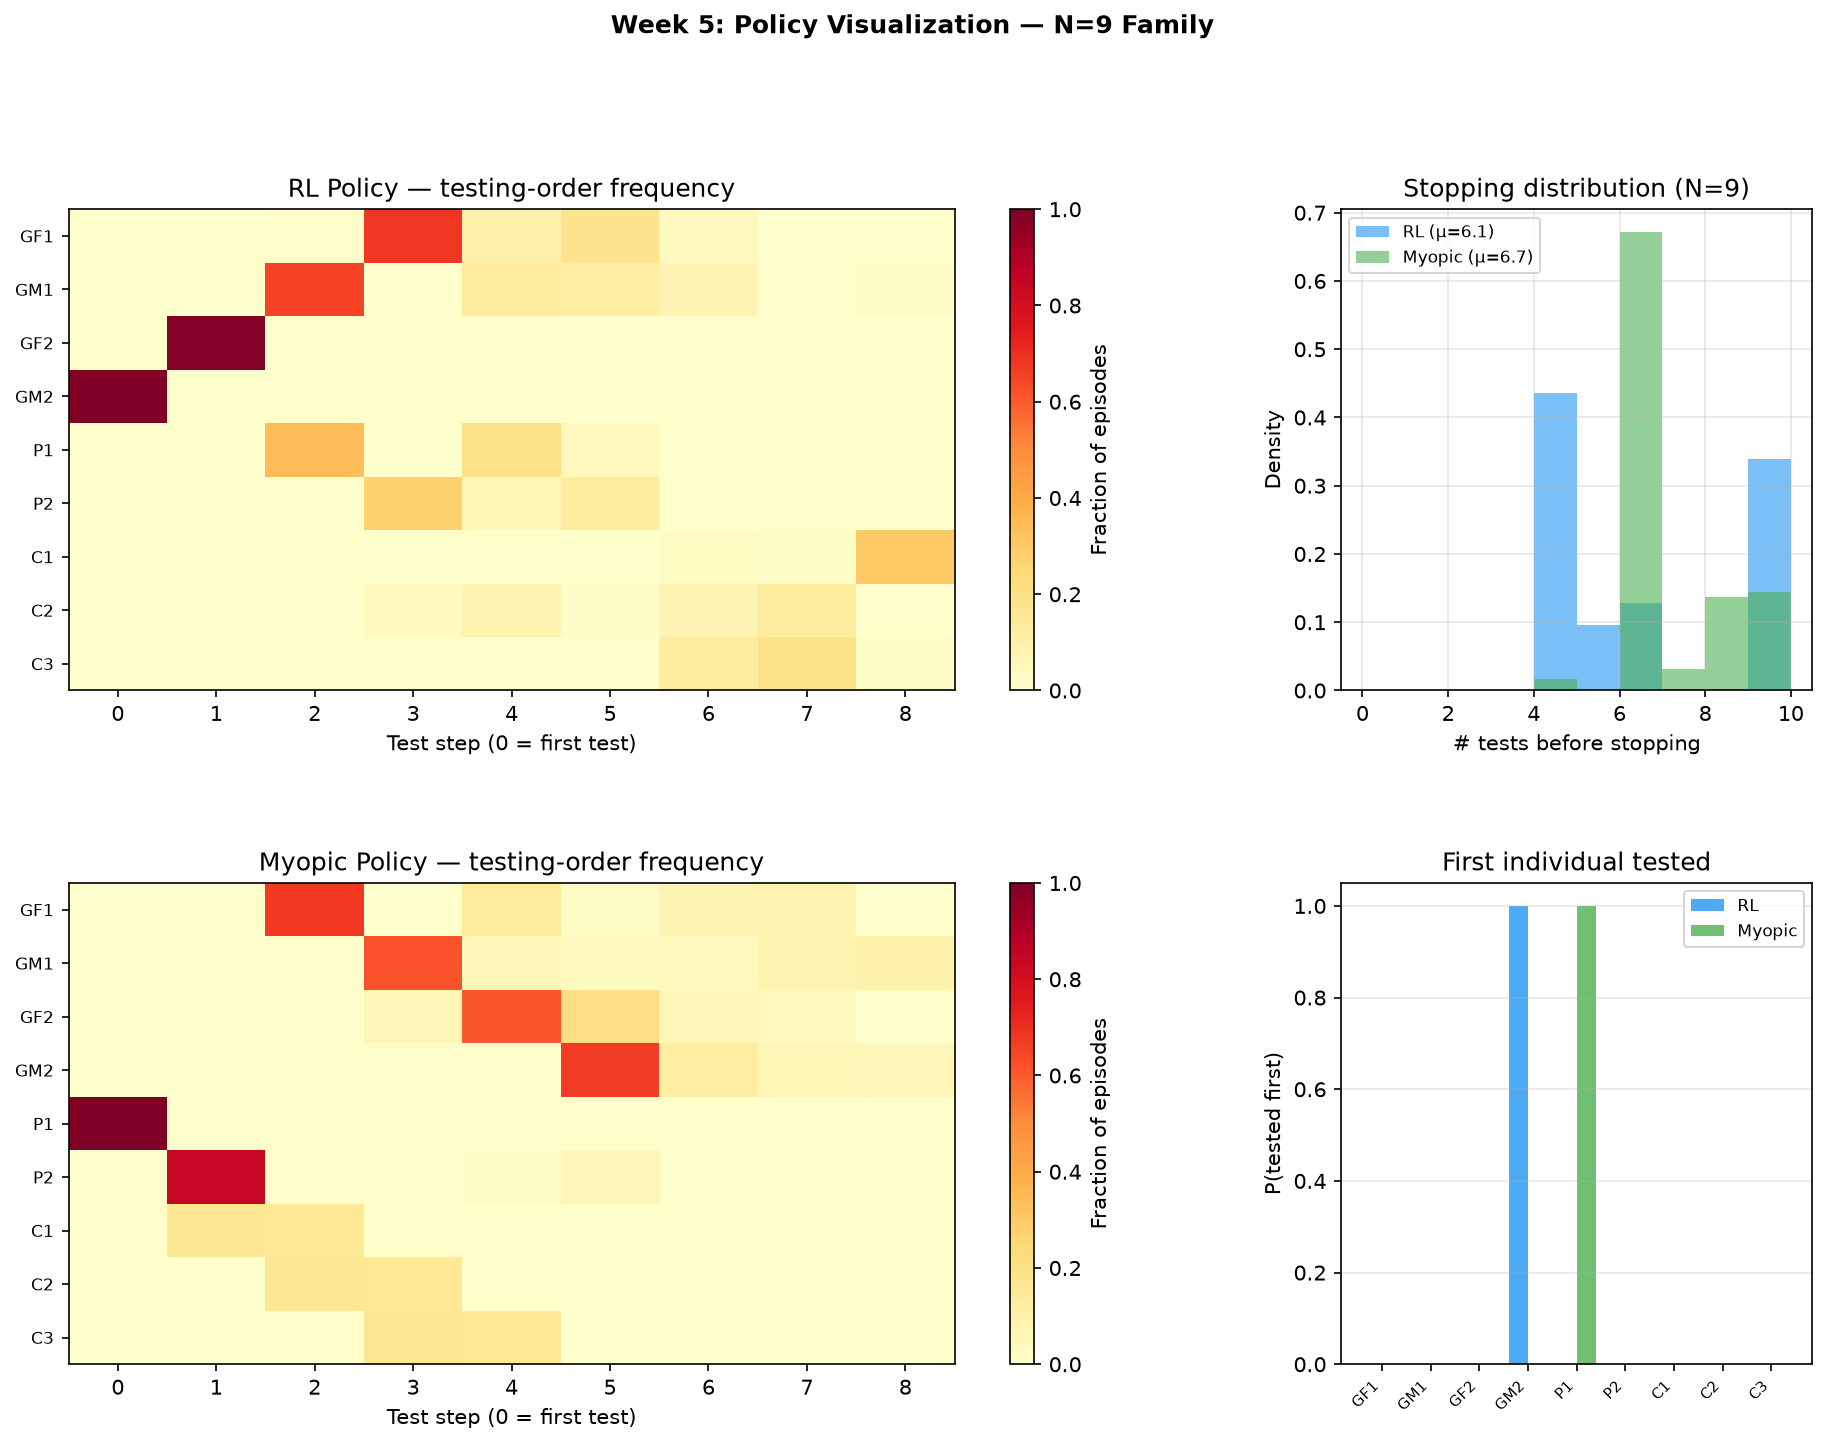
\includegraphics[width=0.65\linewidth]{../artifacts/fig10_policy_viz.png}
  \caption{Policy behaviour: RL vs myopic greedy (2,000 episodes)}
\end{figure}

\subsection{6 — ABCD-16 Replication: Validating Our Solver}
\textit{Script: \texttt{replicate.py}}

Re-ran the lab's existing ABCD-16 model on 4 named families from the original report.
Compared reproduced ratio2/ratio3 to published numbers.

\textbf{Why:} if our exact DP solver is wrong, every gap number above is meaningless.
Replicating ABCD-16 to exact precision confirms the solver is correct.

\textbf{Result:} all 4 families reproduced with diff = $+0.00 \times 10^{0}$ —
exact to every digit, far inside the $10^{-6}$ tolerance gate.

\begin{center}
\small
\begin{tabular}{lrr}
\toprule
\textbf{Family} & \textbf{ratio2 (policy gap)} & \textbf{ratio3 (certificate gap)} \\
\midrule
ThreeGeneration\_LowHigh\_Aggressive         & 5.1\%  & 10.7\% \\
Extended\_LowHigh\_Base                      & 10.1\% & 26.8\% \\
Extended\_MediumEven\_Base                   & 15.9\% & 18.8\% \\
Extended\_LowHigh\_Base (phase6)             & 42.3\% & 39.3\% \\
\bottomrule
\end{tabular}
\end{center}

%------------------------------------------------------------------
\section{What Is Still Missing}

\begin{itemize}
  \item \textbf{RL vs ABCD-16 head-to-head} — both methods were never run on the
        same families. Cannot currently claim RL beats ABCD-16 with data.
  \item \textbf{Train on a distribution of families} — RL currently trains
        separately per family size. A proper generalising agent trains on randomly
        sampled families and transfers.
  \item \textbf{Quality metric at N=12, 15} — RL runs at those sizes but we have
        no ground truth to grade it against (exact DP is infeasible).
        Need an alternative evaluation (e.g.\ compare to ABCD-16 or myopic).
  \item \textbf{Statistical significance} — results are over 500 episodes.
        Confidence intervals and significance tests needed before strong claims.
\end{itemize}

\end{document}
